\subsection{Experiment 1: the Lyapunov profile of the residual stream over training (clocks 1 and 2)}
\label{sec:exp1}

\paragraph{Question and setup.} Finite-time Lyapunov exponents \eqref{eq:ftle} describe how a forward pass stretches perturbations, layer by layer. How does this profile change as the model trains? This question couples clock~1 to clock~2 (\op{1}). We use the public training checkpoints of Pythia \citep{biderman2023pythia}: eleven checkpoints of Pythia-70M (6 layers), from initialization to step 143{,}000, and six checkpoints of Pythia-160M (12 layers). Each block is treated as a map $F_\ell$ on the full residual stream of a 16-token context. For each block we estimate the largest singular value $\sigma_\ell$ of its Jacobian by power iteration and report the relative exponent
\begin{equation}
\tilde\Lambda_\ell=\log\sigma_\ell-\log\big(\|x^{\ell+1}\|/\|x^{\ell}\|\big),
\end{equation}
which measures stretching beyond the growth of the residual norm. For the whole stack we report $\Lambda=\frac{1}{L}\log\sigma_{\max}(\mathrm{D}F_{0\to L})$, and the ratio $\kappa=\log\sigma_{\max}(\mathrm{D}F_{0\to L})/\sum_\ell\log\sigma_\ell$. Since $\sigma_{\max}$ of a product is at most the product of the $\sigma_\ell$, $\kappa\le1$ whenever $\sum_\ell\log\sigma_\ell>0$, which holds throughout our measurements, and $\kappa$ near one means that the most expanded direction of each layer is passed on to the next. Values are means over eight prompts, and $\kappa$ is the ratio of the two means.

\paragraph{Results.} Figure~\ref{fig:exp1} shows three things. First, at initialization both models have the same profile, decreasing with depth ($\tilde\Lambda_\ell$ from 1.20 to 0.53 in Pythia-70M and from 1.19 to 0.39 in Pythia-160M), which reflects the shared initialization scheme. Second, training makes every layer more expansive. The mean of $\tilde\Lambda_\ell$ over layers rises from 0.75 to 2.32 in Pythia-70M and from 0.59 to 2.17 in Pythia-160M, and it is still rising at the last checkpoint. The rise is not monotone at first: at step 128 the deepest layers of Pythia-70M contract further (layer 6 drops from 0.53 to 0.22) before all layers expand. Third, the whole stack does not follow. In Pythia-70M, $\Lambda$ goes from 0.87 to about 1.1 and stays between 1.11 and 1.18 from step 4{,}000 onward, which is under 3\% of training. In Pythia-160M it moves from 0.45 to 0.58. As a result the coherence $\kappa$ falls during training, from 0.67 to 0.36 in Pythia-70M and from 0.52 to 0.22 in Pythia-160M.

\paragraph{Reading.} Training produces layers that are individually more sensitive to perturbations, while the expanding directions of consecutive layers become less aligned, so the forward pass as a whole stretches perturbations only moderately. The depth-averaged exponent settles early, while the per-layer exponents keep changing. This is consistent with the observation that the normalized singular value spectra of the weights stabilize early in pretraining \citep{zhang2026stability}, now seen through the Jacobians of the forward map. These are measurements on two small models with short contexts and a small prompt set. Whether the same pattern holds at scale, and whether $\kappa$ predicts robustness to perturbations or the success of model editing, is part of \op{1}.

\begin{figure}[t]
\centering
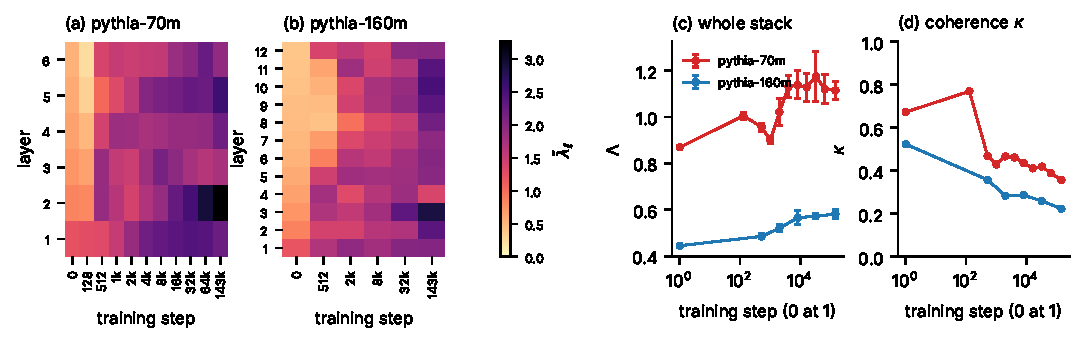
\includegraphics[width=\textwidth]{figs/exp1_ftle.pdf}
\caption{Experiment 1: finite-time Lyapunov exponents of the residual stream across public Pythia checkpoints. (a, b) Relative per-layer exponent $\tilde\Lambda_\ell$ (stretching of the top singular direction beyond the growth of the residual norm) for each layer and checkpoint. (c) Depth-averaged exponent of the whole stack, $\Lambda$; bars: standard deviation over prompts. (d) Coherence $\kappa$ between per-layer and whole-stack stretching; values below one mean that the most expanded directions of consecutive layers are not aligned.}
\label{fig:exp1}
\end{figure}
